\documentclass[12pt, letterpaper]{article}
\usepackage[utf8]{inputenc}
\usepackage[letterpaper]{geometry}
\geometry{top=1.5cm, bottom=2.5cm, left=2.5cm, right=2.5cm}
\usepackage{fancyhdr}
\usepackage{graphicx}
\pagestyle{fancy}
\fancypagestyle{plain}{}
\fancyhf{}
\lfoot[]{Inteligencia Artificial}
\rfoot[]{Enero - Junio 2025}
\renewcommand{\headrulewidth}{0pt}
\renewcommand{\footrulewidth}{1pt}
\usepackage{amsmath,amssymb}
\title{Regresión Lineal en Python}
\author{Aldo Hernández}
\date{Marzo 2025}

\begin{document}
    \maketitle
    \section{Introducción}
    La regresión lineal es un algoritmo usado ampliamente en la estadística y el aprendizaje automático para hacer predicciones y mostrar tendencias a partir de un conjunto de datos, se basa en hacer una función lineal que indica la tendencia del conjunto y hacer predicciones a partir de ella. \par
    La función se puede representar matemáticamente de la siguiente manera
    \begin{equation*}
        y = \beta_{0} + \beta_{1}x_{1} + \beta_{2}x_{2} + \dots + \beta_{n}x_{n}
    \end{equation*}
    donde $\beta_{i}$ representa el coeficiente de la variable independiente $x_{i}$ y $x_{i}$ representa una variable explicativa $i$ (nuestra etiqueta de interés). \par
    La regresión lineal en el aprendizaje automático es un algoritmo que se puede clasificar como de aprendizaje supervisado ya que obtiene por sí mismo la función lineal que muestra la tendencia de nuestros datos.
    \section{Metodología}
    Primero, se importan los paquetes necesarios para la actividad y las configuraciones necesarias para ajustar el tamaño y estilo de los gráficos
    \begin{center}
        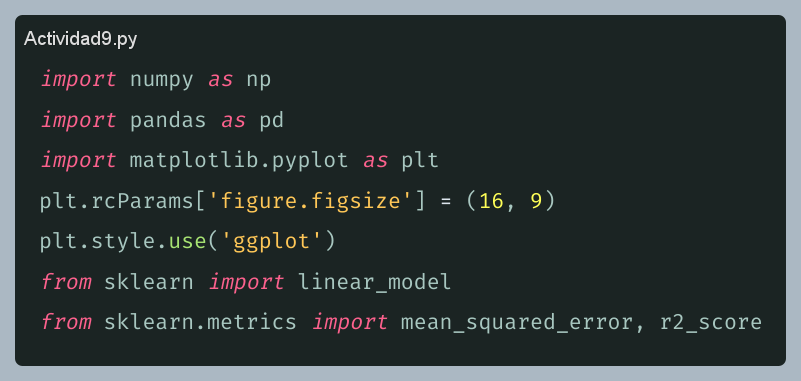
\includegraphics[width=90mm]{2025-03-23-22-52-59.png}
    \end{center}
    Después, se leen los datos desde un archivo csv con pandas para procesarlo como un dataframe y eliminan las columnas que no son de interés
    \begin{center}
        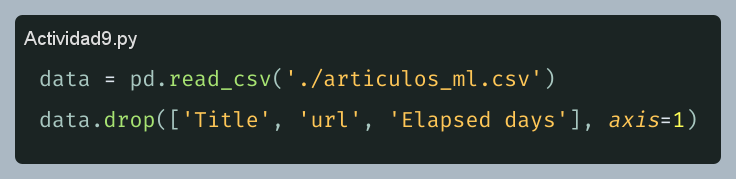
\includegraphics[width=90mm]{2025-03-23-23-20-45.png}
    \end{center}
    Como primer parte de la actividad, solo hay que filtrar los datos para que se ajusten a la mayoría de la información que tenemos; se usan dichas condiciones debido a que previamente se analizó el conjunto de datos mediante histogramas y se concluyó que la mayoría de datos se concentraba dentro de dichos filtros, con esto eliminamos posibles anomalías según nuestros datos. Luego le asignamos colores a la mitad sobre la media de palabras y a la mitad debajo de dicha media
    \begin{center}
        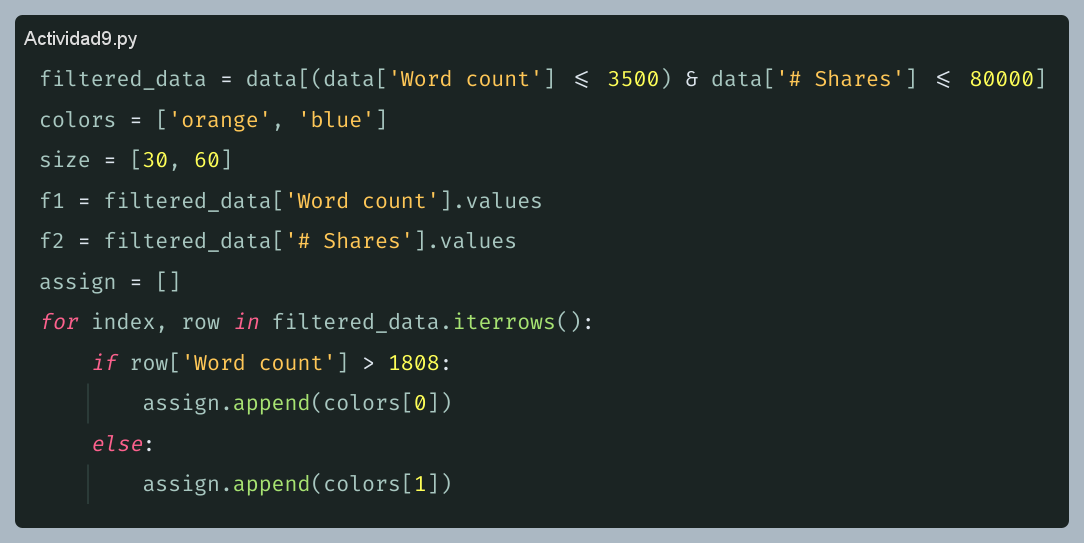
\includegraphics[width=140mm]{2025-03-23-23-24-51.png}
    \end{center}
    Continuando con la actividad, creamos un nuevo dataframe con nuestras dos etiquetas de interés: conteo de palabras y suma de enlaces, comentarios e imágenes o videos. Posteriormente creamos un modelo de regresión lineal múltiple que se ajuste a ambas etiquetas y nuestra salida (el número de compartidos) e imprimimos su información: los coeficientes lineales, el error cuadrado promedio como medida de eficacia y el puntaje de varianza.
    \begin{center}
        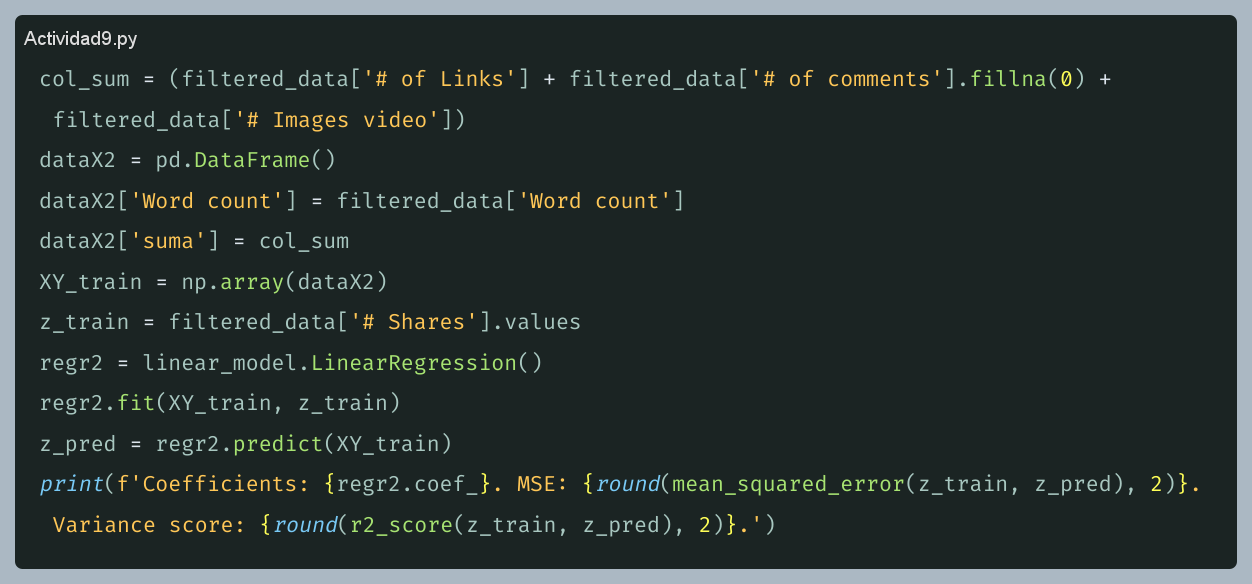
\includegraphics[width=160mm]{2025-03-23-23-30-04.png}
    \end{center}
    Finalmente, solo queda crear la gráfica en 3d; para ello, creamos una figura y una malla sobre la que representaremos nuestros datos, luego ajustamos nuestros vectores.
    \begin{center}
        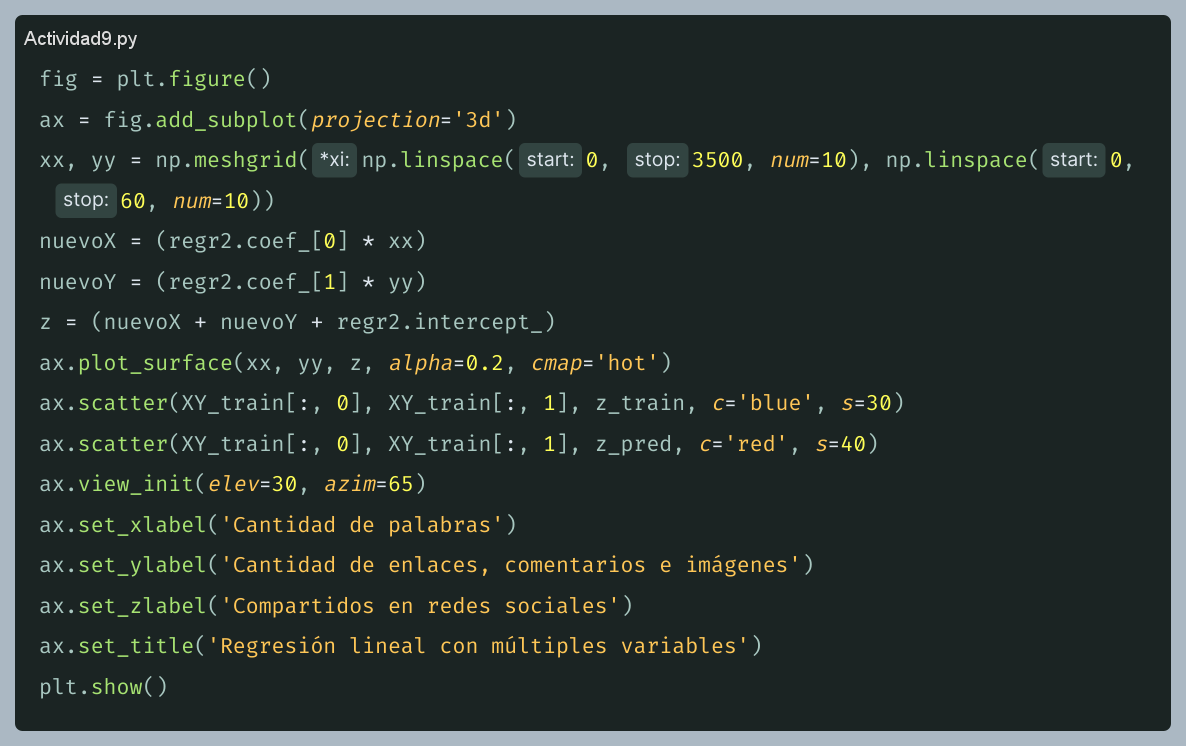
\includegraphics[width=140mm]{2025-03-23-23-34-21.png}
    \end{center}
    \begin{center}
        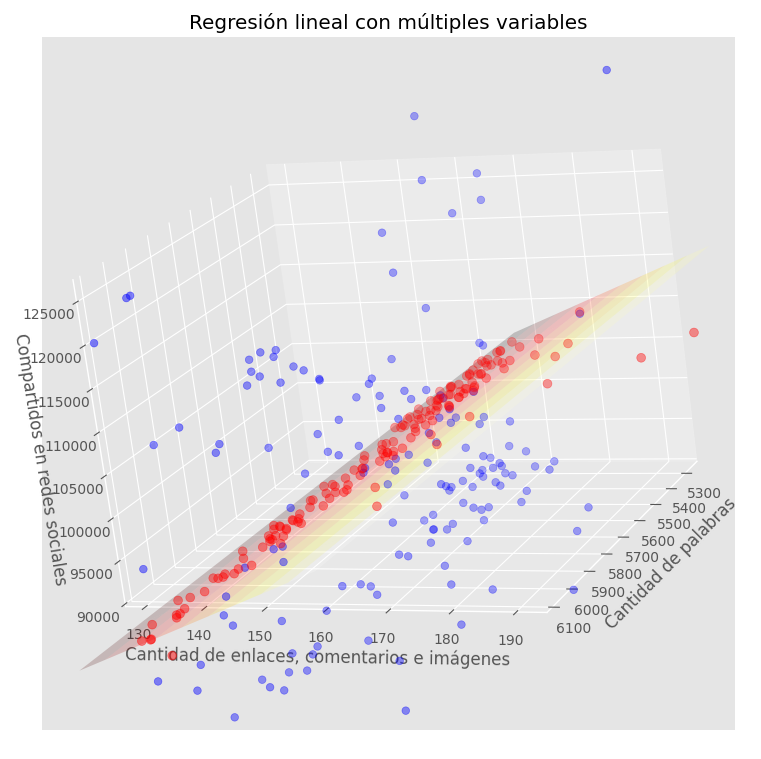
\includegraphics[width=140mm]{2025-03-23-23-36-29.png}
    \end{center}

    \section{Resultados}
    A pesar de que según las métricas utilizadas sugieren que el modelo no es confiable, podemos hacer unas cuantas predicciones según la función generada
    \begin{equation*}
        z = 21140.97 + 0.493x_{1} + 289.3253x_{2}
    \end{equation*}
    Por ejemplo, si tenemos un artículo con 2000 palabras, 10 enlaces, 4 comentarios y 6 imágenes, deberiamos tener aproximadamente 27913 compartidos según la siguiente predicción:
    \begin{equation*}
        z = 21140.97 + 0.493(2000) + 289.3253(10+4+6) \approx 27913
    \end{equation*}

    \section{Conclusión}
    Este algoritmo es de gran utilidad para notar tendencias según nuestras características de interés, sin embargo, pierde mucho valor si no se ajusta bien a nuestros datos ya que puede llevarnos a predicciones erróneas. Es por esto que en mi opinión, la regresión lineal debería utilizarse sólo cuando se quiere ver la tendencia según ciertas características o si tenemos un conjunto demasiado grande de datos para evitar el underfitting. \par
    Además, se puede ganar mucho valor de este algoritmo si se combina con alguna técnica de reducción de dimensionalidad como el SVD porque con ambos podemos comprender mejor el conjunto de datos que tenemos y nos puede mostrar mejor las tendencias usando menos etiquetas.
\end{document}